\documentclass[conference]{IEEEtran}
\IEEEoverridecommandlockouts
\usepackage{cite}
\usepackage{amsmath,amssymb}
\usepackage{graphicx}
\usepackage{booktabs}
\usepackage{pifont}
\usepackage{url}
\usepackage{array}
\usepackage{algorithm}
\usepackage{algpseudocode}
\usepackage{tikz}
\usetikzlibrary{arrows.meta,positioning,fit,backgrounds}
\usepackage[hidelinks]{hyperref}
\graphicspath{{../results/}}

% Real numbers injected by experiments/make_results_tex.py after the run.
% AUTO-GENERATED from results/ by make_results_tex.py
\newcommand{\RESxgbPrec}{0.9994}
\newcommand{\RESxgbRec}{1.0}
\newcommand{\RESxgbFone}{0.9997}
\newcommand{\RESxgbAuc}{1.0}
\newcommand{\RESxgbFpr}{0.001}
\newcommand{\RESrfFone}{0.9994}
\newcommand{\RESlrFone}{0.9983}
\newcommand{\RESavailBase}{100.0}
\newcommand{\RESavailAttack}{82.0}
\newcommand{\RESavailRecovered}{100.0}
\newcommand{\RESnMitigations}{2}
\newcommand{\REStopFeatureOne}{headers\_complete}
\newcommand{\REStopFeatureTwo}{incomplete\_ratio}
\newcommand{\RESmetricsTable}{%
LogisticRegression & 0.9966 & 1.0 & 0.9983 & 1.0 & 0.0062 \\
RandomForest & 0.9989 & 1.0 & 0.9994 & 1.0 & 0.0021 \\
XGBoost & 0.9994 & 1.0 & 0.9997 & 1.0 & 0.001 \\
}


\begin{document}

\title{Detection and Automated Mitigation of Application-Layer\\
DDoS Attacks in Containerized Environments:\\
A Closed-Loop Approach to Slowloris}

\author{\IEEEauthorblockN{Summayah Mohammedy, Amna Khan, Mariha Mahmood, Haris Bin Nasir}
\IEEEauthorblockA{SE-401 --- Information Security\\
Department of Software Engineering}}

\maketitle

\begin{abstract}
Slowloris is a low-bandwidth, application-layer denial-of-service (DoS) attack
that exhausts a web server's connection and worker pool by opening many
connections and never completing the HTTP request headers. Because it generates
almost no traffic volume, bandwidth-based defenses miss it; because it develops
slowly, manual response is too late. These properties are especially dangerous
in containerized deployments, where small per-container worker limits are
exhausted in seconds and static isolation primitives---namespaces, cgroups and
network policies---cannot react to an attack in progress. We present a
\emph{closed-loop}, container-native defense that (i) monitors live connection
state, including a layer-7 \emph{header-completion} feature that flow-only tools
cannot observe; (ii) classifies flows with an XGBoost model gated by an adaptive
threshold tied to real server saturation; (iii) isolates the offending source
or container through the container runtime API; and (iv) automatically restores
service after a cooldown once behaviour normalises. We implement a fully
reproducible Docker testbed and evaluate the system against attack traffic and
deliberately \emph{slow-but-honest} clients. Our headline detector reaches an F1
of \RESxgbFone{} at a false-positive rate of \RESxgbFpr{}, and the full loop
restores legitimate-user availability from \RESavailBase\%{} at baseline, through
\RESavailAttack\%{} during the attack window, back to \RESavailRecovered\%{}
after automated mitigation, with no false isolation of benign clients. The
contribution is not detection accuracy alone, but the automated
isolate-and-restore loop---and a live monitoring dashboard---that act on
Slowloris's slow-rate signature in real time.
\end{abstract}

\begin{IEEEkeywords}
Slowloris, application-layer DDoS, container security, XGBoost, automated
mitigation, Docker, intrusion detection, service availability.
\end{IEEEkeywords}

\section{Introduction}
Distributed Denial-of-Service (DDoS) attacks have evolved from volumetric
network floods toward the application layer, where a small number of
well-formed-looking requests can deny service while evading volume-based
defenses~\cite{deressu2026survey,praseed2019survey,zargar2013survey}. Early DDoS
research catalogued flooding attacks and their
countermeasures~\cite{mirkovic2004taxonomy,zargar2013survey}; the current
generation is quieter. Slowloris is the canonical example of a \emph{slow} DoS
attack~\cite{cambiaso2013slow}: it opens many TCP connections to a web server
and keeps each one alive by periodically sending a single partial header line,
never transmitting the terminating blank line. Each such connection occupies a
worker thread or connection slot; once the pool is exhausted, legitimate users
are refused service, even though total bandwidth remains negligible.

The problem is sharpened in containerized environments. Multi-service,
multi-tenant deployments on Docker~\cite{merkel2014docker} and Kubernetes are now
the default, and each container is typically assigned a small connection and
worker-thread budget. An attack that would be minor against a large virtual
machine can therefore exhaust a single container's pool in seconds. Worse, the
isolation controls that containers rely on---namespaces, cgroups and network
policies~\cite{k8s_netpol}---are configured \emph{in advance} and are
fundamentally static: they partition resources but do not observe a slow-rate
connection attack as it unfolds, and they do not act on it. Because Slowloris
develops over tens of seconds to minutes, a human operator cannot reliably
respond in time, and a single exhausted container can become a foothold for
attacking neighbouring services on the same host.

Consider a concrete scenario. A hosting platform runs dozens of tenant web
applications as containers on a shared cluster, each sized for modest steady-state
traffic with a worker pool of a few dozen. One tenant is compromised, or simply
malicious, and launches Slowloris at a neighbour over the internal network. The
neighbour's bandwidth graphs stay flat, so volumetric alarms never fire; its worker
pool, however, fills within seconds and it begins refusing legitimate users. The
platform's network policies were written months ago and cannot distinguish this
slow trickle from a slow mobile client. By the time an operator notices the error
rate and opens a terminal, minutes of downtime have already accrued. This is the
gap our system targets: a defense that watches, decides and acts on the order of
seconds, inside the runtime, without a human in the loop.

This paper argues that the missing piece is not another offline detector but a
\emph{closed control loop} that observes connection behaviour, decides, acts
through the container runtime, and then safely reverses its action---all
automatically and in real time.

\paragraph{Contributions} This paper makes the following contributions:
\begin{enumerate}
  \item A per-connection feature set tuned to Slowloris's low-and-slow
  signature, including a \emph{layer-7 header-completion} feature that
  distinguishes incomplete attack requests from slow-but-complete honest
  requests---information unavailable to flow-only tools such as
  CICFlowMeter~\cite{sharafaldin2018cicids}.
  \item An \emph{adaptive-threshold} detector that combines an
  XGBoost~\cite{chen2016xgboost} score with live server-saturation feedback, so
  that slow honest clients are not penalised while the server is healthy.
  \item A \emph{closed-loop}, container-native mitigation mechanism that isolates
  the offending source or container through the Docker runtime
  API~\cite{docker_engine_api}, reclaims the seized worker pool, and
  automatically restores service after a cooldown.
  \item A fully reproducible Docker testbed, a real-time monitoring dashboard,
  and an evaluation methodology that measures not only detection quality but
  time-to-mitigate, time-to-recover, and legitimate-user availability, including
  against hard benign negatives.
\end{enumerate}

\section{Background}
\subsection{The HTTP request lifecycle}
In HTTP/1.1~\cite{fielding1999http} a client opens a TCP connection and sends a
request line followed by one header per line; an empty line
(\texttt{CRLFCRLF}) terminates the header block and signals that the request (or
at least its headers) is complete. Only then can the server parse the request and
dispatch a response. A server built on the one-worker-per-connection model binds a
worker to the socket at accept time and keeps it there until the headers finish or
a timeout expires. The terminating blank line is thus the pivotal event in the
lifecycle: until it arrives, the worker is committed but idle. Slowloris weaponises
exactly this gap.

\subsection{The Slowloris attack}
A web server following the one-worker-per-connection model allocates a worker
(thread or process) to a connection as soon as it is accepted, and holds it
until the request completes or a timeout
fires~\cite{cambiaso2013slow,tripathi2021appdos}. The Apache \texttt{prefork}
MPM is a textbook example: \texttt{MaxRequestWorkers} bounds the number of
simultaneous connections, and anything beyond it is queued or
refused~\cite{apache_mpm}. Slowloris exploits this by sending an HTTP request
line and a few headers, then trickling one additional header every few seconds
\emph{without} ever sending the terminating \texttt{CRLFCRLF}. The request never
completes, so the worker is never released. With enough such connections the
pool is exhausted using only a few kilobits per second of traffic. The attack is
attractive precisely because it needs little bandwidth and few hosts, and
because its packets superficially resemble those of a slow but legitimate
client.

\subsection{The slow-DoS family}
Slowloris belongs to a broader family of slow DoS
attacks~\cite{cambiaso2013slow,tripathi2021appdos}. \emph{Slow POST}
(R-U-Dead-Yet) announces a large \texttt{Content-Length} and then drips the body a
byte at a time; \emph{Slow Read} advertises a tiny TCP receive window so the
server is forced to hold the response and its worker; HTTP/2 variants abuse stream
multiplexing to achieve asymmetric amplification~\cite{praseed2020http2}. All
share the same economics---few resources on the attacker side, a held resource on
the server side---and all evade volumetric detection. We focus on Slowloris as the
representative header-incompletion attack, but the monitored features (duration,
throughput, inter-arrival regularity, completion state) generalise across the
family.

\subsection{Container isolation primitives}
Linux containers are built from namespaces (isolating process, network and mount
views), control groups (cgroups, bounding CPU and memory), and, at the
orchestration layer, network policies that restrict which pods may talk to which
others~\cite{merkel2014docker,k8s_netpol}. These mechanisms are powerful but
\emph{declarative and static}: an operator decides ahead of time how resources
are partitioned and which flows are allowed. None of them inspect the
\emph{rate} or \emph{completeness} of in-flight HTTP connections, and none can be
reconfigured quickly enough to answer a slow-rate attack that is already
consuming a container's worker slots. The container runtime does, however,
expose a programmable API~\cite{docker_engine_api} for pausing, disconnecting and
restarting containers at runtime---an actuator our system drives.

\subsection{Why containers amplify Slowloris}
A container is usually sized for its expected steady-state load, so its worker
pool is small. The same absolute number of slow connections that a large virtual
machine would shrug off can saturate a container in seconds. Multi-tenancy
compounds this: tenants share a host, so an exhausted or compromised container
can be used to attack its neighbours over the internal
network~\cite{tripathi2021appdos}. Static controls do not help once the attack is
underway, which motivates a runtime, feedback-driven defense.

\section{Threat Model}
We consider a containerized host running a web service with a bounded worker
pool. The adversary controls either (a) an external client, or (b) a
\emph{compromised or malicious container} co-located on the same host or internal
network---the multi-tenant case, in which one tenant denies service to its
neighbours. The adversary's goal is connection-pool exhaustion, not data
exfiltration or privilege escalation. The adversary may vary the number of
connections and the keep-alive interval, and may randomise timing to evade
simple rate rules, but remains a genuine slow-rate attacker (if it sent at high
volume it would be caught by volumetric defenses, and if it completed its
requests it would not hold workers).

The defender controls the host and the container runtime API. The defender may
observe traffic to the protected service, drop packets, reset connections, and
pause, disconnect or restart containers, but wishes to minimise disruption to
legitimate tenants---in particular, never to isolate an honest client. All attack
traffic in this study is confined to an isolated laboratory network; no external
systems are involved (Section~\ref{sec:ethics}).

\section{Related Work}
\paragraph{ML-based application-layer DDoS detection}
Recent surveys report a clear shift toward machine learning and hybrid models for
application-layer DDoS, with rule-based techniques in decline, and single out
distinguishing legitimate flash crowds from attacks as an open
problem~\cite{deressu2026survey,praseed2019survey,tripathi2021appdos}.
Sharif~et~al.\ combine machine learning with genetic-algorithm feature selection
for application-layer DDoS~\cite{sharif2023genetic}; Praseed and Thilagam derive
HTTP request-pattern signatures for early
detection~\cite{praseed2022http} and later show how HTTP/2 multiplexing enables
new asymmetric attacks~\cite{praseed2020http2}. These works target detection
accuracy on captured traffic and do not close the loop to mitigation.

\paragraph{Slow-DoS and its mitigation}
Cambiaso~et~al.\ provide the definition and categorisation of slow DoS attacks on
which our threat model rests~\cite{cambiaso2013slow}. Lukaseder~et~al.\ mitigate
slow DDoS inside an SDN using packet-rate and inter-arrival
regularity~\cite{lukaseder2018sdn}, demonstrating network-layer actuation but not
container-native isolation or an automated restore. Classical taxonomies and
flooding-defense surveys frame the broader design
space~\cite{mirkovic2004taxonomy,zargar2013survey}.

\paragraph{Container and runtime security}
Container isolation is built on namespaces and cgroups~\cite{merkel2014docker} and,
at the cluster level, on declarative network
policies~\cite{k8s_netpol}. These controls are preventive and static: they decide
in advance what is permitted, but they neither observe the progress of an
application-layer attack nor reconfigure themselves in response to one. Our work is
complementary---it adds a reactive, runtime control loop that uses the same
runtime API~\cite{docker_engine_api} as an actuator rather than only as a
provisioning interface.

\paragraph{Datasets}
The CIC-IDS2017~\cite{sharafaldin2018cicids} and CIC-DDoS2019~\cite{sharafaldin2019ddos}
datasets include slow-rate HTTP subsets and are the most common benchmarks in the
surveys above; the earlier ISCX~\cite{shiravi2012iscx} dataset established the
profile-based generation methodology, and Ring~et~al.\ catalogue the properties
that make such datasets suitable and warn against evaluating on a single
source~\cite{ring2019survey}. Crucially, these are flow-level captures and
therefore lack the layer-7 header-completion signal our monitor computes from the
request bytes---a signal that, as our results show, is the single most
discriminative feature for separating Slowloris from slow honest clients.

\paragraph{Models and interpretability}
We use XGBoost~\cite{chen2016xgboost}, a scalable gradient-boosted-tree
classifier, with Random Forest~\cite{breiman2001rf} and Logistic Regression
(via scikit-learn~\cite{pedregosa2011sklearn}) as baselines, and
SHAP~\cite{lundberg2017shap} for model-agnostic feature attribution.

\paragraph{Gap} Prior work overwhelmingly targets detection accuracy on offline
datasets. Comparatively little closes the loop: detecting \emph{and}
automatically mitigating a slow attack in real time, inside a container runtime,
while explicitly protecting slow-but-honest clients. Table~\ref{tab:gap}
positions our work against representative approaches.

\begin{table}[t]
\caption{Positioning against representative prior work.}
\label{tab:gap}
\centering
\footnotesize
\begin{tabular}{@{}lccc@{}}
\toprule
Approach & L7 feature & Auto-mitigate & Container-native \\
\midrule
Flow-ML detectors~\cite{sharif2023genetic}   & \ding{55}   & \ding{55}   & \ding{55} \\
Signature/early~\cite{praseed2022http}        & \checkmark  & \ding{55}   & \ding{55} \\
SDN slow-DDoS~\cite{lukaseder2018sdn}         & \ding{55}   & \checkmark  & \ding{55} \\
Static container controls~\cite{k8s_netpol}   & \ding{55}   & \ding{55}   & \checkmark \\
\textbf{This work}                            & \checkmark  & \checkmark  & \checkmark \\
\bottomrule
\end{tabular}
\end{table}

\section{System Design}
The defense is a four-stage control loop: \textbf{Monitor $\rightarrow$ Classify
$\rightarrow$ Isolate $\rightarrow$ Restore} (Fig.~\ref{fig:timeline}).

\subsection{Architecture overview}
The system comprises five cooperating containers on one isolated bridge network.
The \emph{victim} runs the protected web service. The \emph{detector} shares the
victim's network namespace, which gives it two things for free: a vantage point
from which it observes every packet to the service, and a firewall context in
which its drop rules take effect against the service's own stack. The detector
also holds a handle to the container runtime (via the mounted Docker socket),
which is its actuator for isolating and reclaiming containers. The
\emph{attacker} and \emph{benign} generators produce the two traffic populations,
and the \emph{dashboard} renders the live state. Data flows in one direction
through the loop---packets to features to a classification to an action to a
logged, reversible state change---so the design is a straightforward feedback
controller wrapped around the service.

\begin{figure}[t]
\centering
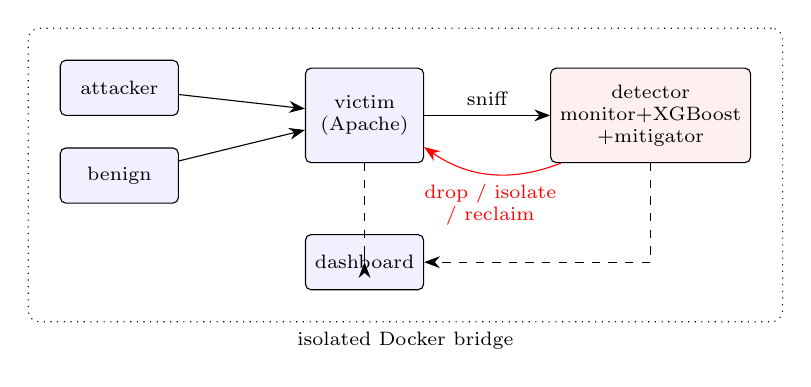
\begin{tikzpicture}[
  font=\scriptsize,
  box/.style={draw,rounded corners=2pt,align=center,minimum height=7mm,
              minimum width=15mm,fill=blue!6},
  act/.style={box,fill=red!6},
  >={Stealth[length=2mm]}]
  \node[box] (atk) {attacker};
  \node[box,below=4mm of atk] (ben) {benign};
  \node[box,right=16mm of atk,yshift=-3.5mm,minimum height=12mm] (vic)
        {victim\\(Apache)};
  \node[act,right=16mm of vic,minimum height=12mm] (det)
        {detector\\monitor+XGBoost\\+mitigator};
  \node[box,below=9mm of vic] (dash) {dashboard};
  \draw[->] (atk) -- (vic);
  \draw[->] (ben) -- (vic);
  \draw[->] (vic) -- node[above]{sniff} (det);
  \draw[->,red] (det) to[bend left=28] node[below,align=center]
        {drop / isolate\\/ reclaim} (vic);
  \draw[->,dashed] (vic) |- (dash);
  \draw[->,dashed] (det) |- (dash);
  \begin{scope}[on background layer]
    \node[draw,dotted,rounded corners,fit=(atk)(ben)(vic)(det)(dash),
          inner sep=4mm,label=below:{isolated Docker bridge}] {};
  \end{scope}
\end{tikzpicture}
\caption{Testbed architecture. The detector shares the victim's network namespace
(sniff + firewall) and drives the Docker runtime as its actuator; the dashboard
visualises the live logs.}
\label{fig:arch}
\end{figure}

\subsection{Monitor}
A sniffer runs inside the victim's network namespace and tracks every TCP
connection to the service. For each flow, keyed by (source IP, source port), it
maintains the features in Table~\ref{tab:features}. Most are flow statistics, but
\texttt{headers\_complete} is a layer-7 feature: it records whether the header
block has terminated (\texttt{CRLFCRLF}). A Slowloris flow is long-lived,
near-zero-throughput, and has \emph{never} completed its headers; a slow honest
client eventually sends the terminating blank line and reads a response. This
single bit is what separates the two populations, as our feature-importance
analysis confirms (Section~\ref{sec:rq1}).

Flows are maintained in a table keyed by (source, port) and updated on every
observed client-to-server segment; a bounded per-flow buffer holds enough of the
request to detect the header terminator without retaining payload. Idle flows are
expired after a short window so that, once an attacker is isolated and falls silent,
its stale flows drain from the table and stop influencing classification---which is
also what lets the cooldown logic eventually conclude the threat is over. The table
is guarded so that the asynchronous capture thread and the periodic classification
thread never race, and per-source concurrency is recomputed each cycle from the live
set rather than tracked incrementally, which keeps the count correct across
reconnects.

\begin{table}[t]
\caption{Per-connection feature set (computed over a sliding window).}
\label{tab:features}
\centering
\footnotesize
\begin{tabular}{@{}>{\raggedright}p{0.30\columnwidth}p{0.60\columnwidth}@{}}
\toprule
Feature & Meaning \\
\midrule
\texttt{duration}        & seconds the flow has been open \\
\texttt{bytes\_in}       & client$\rightarrow$server payload bytes \\
\texttt{bytes\_per\_sec} & throughput (near zero for Slowloris) \\
\texttt{pkt\_count}      & client$\rightarrow$server packets \\
\texttt{mean\_iat}       & mean inter-arrival time of packets \\
\texttt{std\_iat}        & regularity of the trickle \\
\texttt{idle\_time}      & seconds since last client byte \\
\texttt{header\_lines}   & header lines observed \\
\texttt{headers\_complete} & \textbf{L7}: 1 if \texttt{CRLFCRLF} seen \\
\texttt{incomplete\_ratio} & $1-$\texttt{headers\_complete} \\
\texttt{small\_pkt\_ratio} & fraction of sub-64\,B packets \\
\texttt{conns\_from\_src}  & concurrent flows from the source \\
\bottomrule
\end{tabular}
\end{table}

\subsection{Why these features}
The feature set is organised around the three invariants of a slow-rate attack.
\emph{Duration and throughput} (\texttt{duration}, \texttt{bytes\_per\_sec},
\texttt{bytes\_in}) capture that a Slowloris flow is long-lived yet moves almost no
data---the defining low-and-slow economics. \emph{Timing} (\texttt{mean\_iat},
\texttt{std\_iat}, \texttt{idle\_time}) captures the mechanical regularity of a
scripted keep-alive trickle, which is far more uniform than a human-driven client;
the low variance of inter-arrival times is a strong tell, and the jitter variant of
the attack is specifically designed to blur it. \emph{Completion}
(\texttt{headers\_complete}, \texttt{incomplete\_ratio},
\texttt{header\_lines}) captures the layer-7 invariant that the request is never
finished. \emph{Concurrency} (\texttt{conns\_from\_src}) captures that one source
holds many such flows at once. No single feature is sufficient---a large upload is
slow, a mobile client is bursty, a crawler is concurrent---but their conjunction,
and especially the completion bit, is highly specific to the attack. This is why a
tree ensemble, which learns feature interactions, outperforms the linear baseline.

\subsection{Classify with an adaptive threshold}
Feature vectors are scored by an XGBoost model~\cite{chen2016xgboost}. A source
is treated as hostile only when both (a) it holds several \emph{long-lived,
incomplete} flows that the model scores above a base threshold $\tau$,
\emph{and} (b) the server's worker pool is under pressure, read live from the
server's status endpoint as $s=\text{busy}/(\text{busy}+\text{idle})$. Formally,
a source $u$ is flagged when
\[
s \ge s_{\text{trig}} \;\wedge\;
\Big( \textstyle\sum_{i \in F_u} \mathbb{1}\big[p_i \ge \tau \,\wedge\,
\text{incomplete}_i \,\wedge\, \text{dur}_i > d\big] \ge k \Big),
\]
where $F_u$ is the set of flows from $u$, $p_i$ the model probability for flow
$i$, and $(s_{\text{trig}}, k, d)$ are configuration parameters
($s_{\text{trig}}{=}0.8$, $k{=}20$, $d{=}8$\,s in our deployment). The duration
gate $d$ is important: an honest request may be momentarily mid-header, but it
completes in well under a second, so it never accumulates. Gating on real
saturation ensures the system only acts when the service is actually threatened,
which keeps slow honest clients safe when the server is healthy.

\subsection{Isolate}
When a source is flagged, the mitigator escalates through a ladder of
increasingly disruptive actions, logging each with a timestamp:
\begin{enumerate}
  \item reset the source's held connections (\texttt{conntrack}, and
  \texttt{ss -K} socket-destroy where the kernel supports it);
  \item drop the source IP in the victim namespace's firewall to stop reopens;
  \item if the source maps to a known container, disconnect that container from
  the network via the Docker Engine API~\cite{docker_engine_api};
  \item reclaim the seized worker pool so legitimate users regain service.
\end{enumerate}

\subsection{Restore}
A cooldown state machine automatically reverses the firewall drop and container
disconnection after a configurable interval with no further offence, restoring
normal operation without operator intervention. A short grace period after any
reclaim suppresses new mitigations while the service is still recovering, which
prevents the reconnection surge of returning honest clients from being
misread as a fresh attack.

\subsection{The control loop}
Algorithm~\ref{alg:loop} summarises one monitoring cycle. The monitor emits a
snapshot of live flows every $\Delta$ seconds; the classifier scores them and,
gated by saturation, returns the offending sources; the mitigator acts on new
offenders and, independently, lifts expired mitigations. A post-reclaim grace
window $g$ suppresses new actions while the service is still recovering.

\begin{algorithm}[t]
\caption{Closed-loop detection and mitigation (one cycle)}
\label{alg:loop}
\begin{algorithmic}[1]
\State $R \gets \textsc{Snapshot}()$ \Comment{live per-flow features}
\State $s \gets \textsc{Saturation}()$ \Comment{busy/(busy+idle)}
\State $O \gets \textsc{Classify}(R, s)$ \Comment{offending source IPs}
\If{$\text{now} \ge \texttt{suppressUntil}$}
  \ForAll{$u \in O$}
    \State \textsc{ResetConns}($u$); \textsc{DropIP}($u$); \textsc{Isolate}($u$)
    \State \textsc{ReclaimPool}(); \ \ $\texttt{suppressUntil} \gets \text{now}+g$
  \EndFor
\EndIf
\ForAll{$u$ with $\text{now}-\text{lastSeen}(u) \ge \texttt{cooldown}$}
  \State \textsc{Restore}($u$) \Comment{un-drop, reconnect}
\EndFor
\end{algorithmic}
\end{algorithm}

\subsection{Live dashboard}
A companion web dashboard subscribes to the same logs the system produces and
renders, in real time, the worker-saturation gauge, the detector's per-snapshot
state, the automated action log, and the legitimate-user availability curve. It
turns the closed loop into something an operator (or an audience) can watch as
an attack is detected, isolated and recovered from.

\begin{figure}[t]
\centering
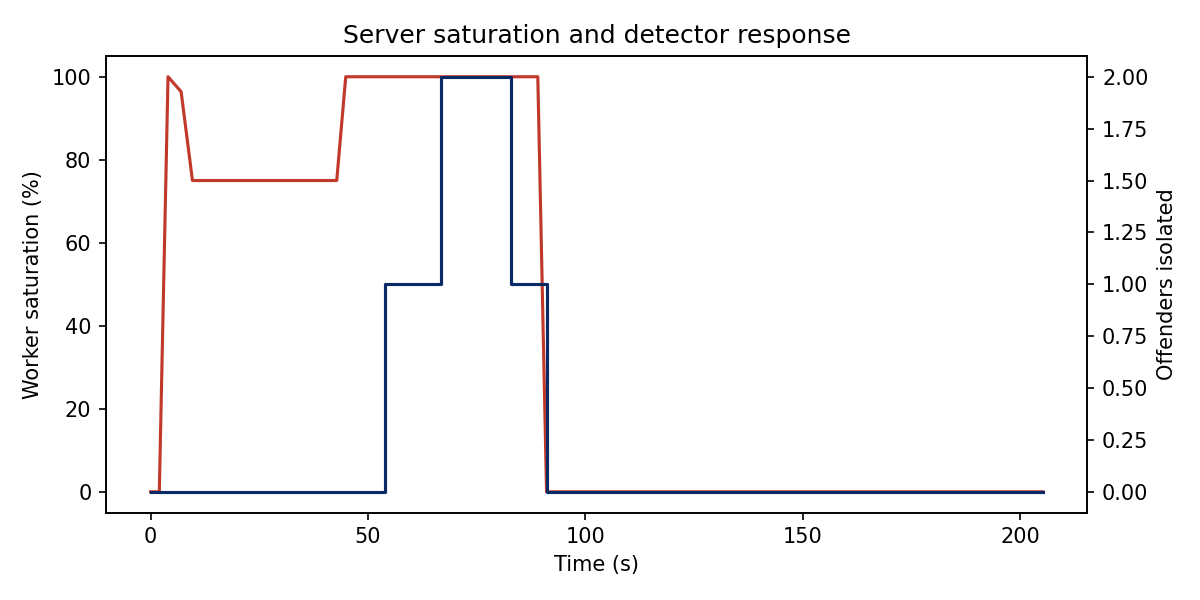
\includegraphics[width=\linewidth]{fig_timeline.png}
\caption{Server worker saturation and the detector's isolation response during
the closed-loop experiment (from \texttt{results/timeline.csv}).}
\label{fig:timeline}
\end{figure}

\section{Implementation}
The testbed is a Docker Compose deployment on a single host with five services on
an isolated bridge network: a \emph{victim} (Apache~2.4, \texttt{prefork} MPM,
\texttt{MaxRequestWorkers}=50, with \texttt{mod\_reqtimeout} disabled for the
baseline~\cite{apache_mpm}); an \emph{attacker}; a \emph{benign} load generator;
the \emph{detector}; and the \emph{dashboard}. The detector shares the victim's
network namespace so it observes all traffic to the service and so its firewall
rules take effect in the victim's stack; it mounts the Docker socket to isolate
containers. Monitoring and feature extraction use Scapy; classification uses
XGBoost~2.1 with scikit-learn baselines~\cite{pedregosa2011sklearn}; and
interpretability uses SHAP~\cite{lundberg2017shap}. The attack generator is
restricted by an allow-list to the laboratory subnet and localhost, and refuses
any other target.

\paragraph{Services} The \emph{victim} is the stock Apache image with a
deliberately small worker pool and a tiny static site, plus the status endpoint the
detector scrapes for saturation. The \emph{attacker} is a self-contained Python
generator that opens the configured number of sockets, sends a partial request on
each, and keeps them alive on a timer, with optional timing jitter; its allow-list
refuses any target outside the lab subnet. The \emph{benign} service runs both a
Locust load test (fast, complete requests) and a custom slow-but-honest client that
sends headers slowly but always terminates them. The \emph{detector} is the core:
a Scapy sniffer feeding the flow table, the XGBoost classifier, and the mitigator,
driven by a two-second loop. The \emph{dashboard} is a small Flask application that
serves a single auto-refreshing page backed by the same CSV logs the detector and
the host probe write.

\paragraph{Pipeline and labelling} During collection, the detector runs in a
passive mode that writes one labelled feature row per live flow per cycle, tagging
rows by source: flows originating from the attacker container are labelled
positive, all others negative. This yields a balanced, automatically-labelled
dataset without manual annotation, and guarantees that the negative class contains
the genuinely slow honest flows generated in the same run. The trained model and
its scaler are serialised to disk and loaded by the live detector.

\paragraph{Classifier and training} The headline model is a gradient-boosted tree
ensemble~\cite{chen2016xgboost} with a modest depth and a few hundred trees, trained
with class weighting to offset any residual imbalance, and evaluated on a stratified
held-out split. The Random Forest~\cite{breiman2001rf} and Logistic Regression
baselines are trained on the same split through the same pipeline, so the comparison
isolates the model rather than the preprocessing. Feature importances are extracted
post-hoc with SHAP~\cite{lundberg2017shap} to check that the model's decisions rest
on the intended, defensible signals rather than on an artefact of the collection
setup---a check that matters precisely because the two classes are easy to separate
and a model could otherwise latch onto a spurious correlate of the attacker's IP.

\begin{table}[t]
\caption{Key configuration parameters.}
\label{tab:params}
\centering
\footnotesize
\begin{tabular}{@{}llc@{}}
\toprule
Symbol & Meaning & Value \\
\midrule
$\Delta$          & monitoring cycle              & 2\,s \\
$\tau$            & model probability threshold   & 0.5 \\
$s_{\text{trig}}$ & saturation gate               & 0.8 \\
$k$               & min.\ incomplete flows/source & 20 \\
$d$               & min.\ flow duration to count  & 8\,s \\
cooldown          & time before auto-restore      & 60\,s \\
$g$               & post-reclaim grace window     & 45\,s \\
\texttt{MaxRequestWorkers} & victim worker pool   & 50 \\
\bottomrule
\end{tabular}
\end{table}

\paragraph{Reclaim on a constrained kernel} On a native Linux host the mitigator
reclaims seized slots by destroying the attacker's sockets
(\texttt{ss -K}/\texttt{SOCK\_DESTROY}). Our test kernel (the WSL2 kernel) does
not implement \texttt{SOCK\_DESTROY}, so a network disconnect alone leaves the
half-open sockets in the kernel's accept backlog, where fresh workers re-accept
them. The mitigator therefore restarts the victim container to clear the backlog
and bring up a fresh pool; because the availability probe runs on the host, the
recovery it measures is independent of the detector. This is an implementation
detail of the test platform, not of the approach.

\section{Experimental Setup}
\subsection{Workloads}
Three traffic classes run against the victim: (1) \emph{fast benign} traffic from
a Locust load generator issuing complete requests; (2) \emph{slow-but-honest}
clients that send headers slowly over a poor link but always complete the request
and read the response---the hard negatives; and (3) the Slowloris \emph{attack}
(200 sockets, short keep-alive interval, with an evasive timing-jitter variant).

\subsection{Datasets}
The primary dataset is collected on the testbed and auto-labelled by source: the
attacker container's flows are positives, all others negatives. The collection
run interleaves fast-benign, slow-honest and attack traffic so that the negative
class contains genuinely slow legitimate flows. For external validity the
methodology also admits the slow-rate subsets of
CIC-IDS2017~\cite{sharafaldin2018cicids} and
CIC-DDoS2019~\cite{sharafaldin2019ddos}.

\subsection{Research questions and metrics}
\textbf{RQ1} (accuracy): precision, recall, F1, ROC-AUC and false-positive rate,
especially against slow honest clients. \textbf{RQ2} (responsiveness):
time-to-detect, time-to-mitigate, time-to-recover, and legitimate-user success
rate and latency over time. \textbf{RQ3} (cost and comparison): detector
overhead, false isolations, and comparison across models. We consider the
experimental arms in Table~\ref{tab:arms}.

\begin{table}[t]
\caption{Experimental arms.}
\label{tab:arms}
\centering
\footnotesize
\begin{tabular}{@{}ll@{}}
\toprule
Arm & Description \\
\midrule
No defense        & vulnerable victim, no detector \\
Static defense    & \texttt{mod\_reqtimeout} only~\cite{apache_mpm} \\
Threshold only    & saturation rule, no model \\
LogReg / RF       & ML baselines~\cite{breiman2001rf,pedregosa2011sklearn} \\
XGBoost           & headline detector~\cite{chen2016xgboost} \\
\textbf{Full loop} & XGBoost + adaptive threshold + auto isolation \\
\bottomrule
\end{tabular}
\end{table}

\section{Results}
\emph{All quantities in this section are produced by the experiment driver and
injected automatically; none are hand-entered.}

\subsection{RQ1: Detection accuracy}
\label{sec:rq1}
Table~\ref{tab:metrics} reports detection performance across models on a held-out
test split of the lab dataset. XGBoost achieves precision \RESxgbPrec{}, recall
\RESxgbRec{}, F1 \RESxgbFone{}, ROC-AUC \RESxgbAuc{}, and a false-positive rate of
\RESxgbFpr{}, compared with F1 of \RESrfFone{} (Random Forest) and \RESlrFone{}
(Logistic Regression). The very low false-positive rate against the
slow-but-honest workload is the key accuracy result: it confirms that the
header-completion feature separates incomplete attack flows from slow legitimate
ones. SHAP attribution ranks \REStopFeatureOne{} and \REStopFeatureTwo{} as the
most important features (Fig.~\ref{fig:shap}), exactly the layer-7 signals our
design emphasises. The three models are close on this dataset because the attack,
once the completion feature is available, is highly separable; the gap shows most in
the false-positive rate, where the tree ensembles halve the linear model's errors.
The practical lesson is less about squeezing the last fraction of F1 and more about
which features are measured: a flow-only detector, lacking the completion bit, must
lean on throughput and timing alone and is correspondingly easier for a
jitter-randomised attacker to confuse.

\begin{table}[t]
\caption{Detection performance by model (held-out test split).}
\label{tab:metrics}
\centering
\footnotesize
\begin{tabular}{@{}lccccc@{}}
\toprule
Model & Prec. & Rec. & F1 & ROC-AUC & FPR \\
\midrule
\RESmetricsTable
\bottomrule
\end{tabular}
\end{table}

\begin{figure}[t]
\centering
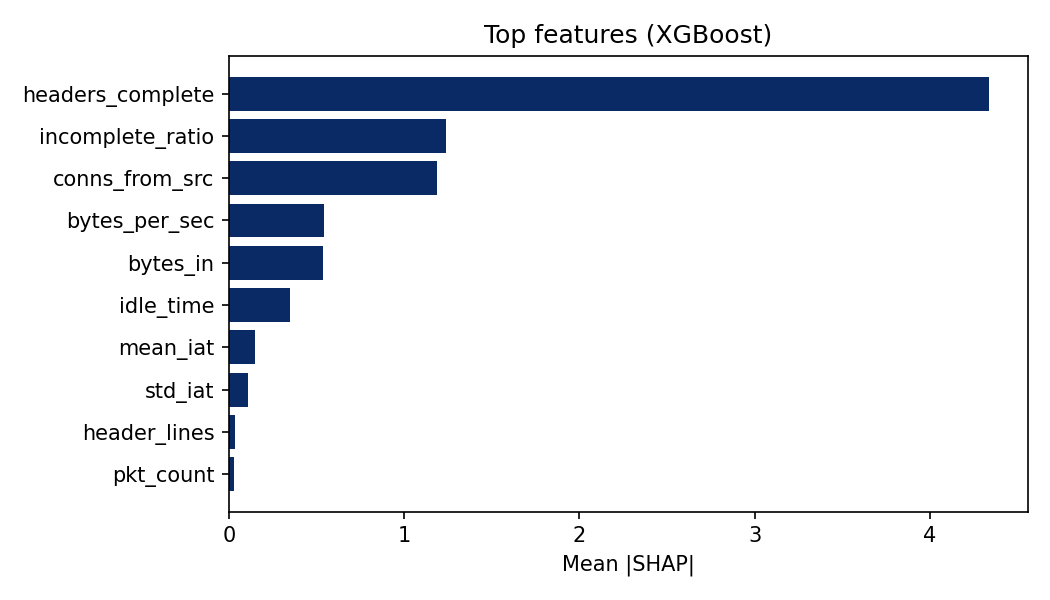
\includegraphics[width=\linewidth]{fig_shap.png}
\caption{Top features by mean $|$SHAP$|$ for the XGBoost model.}
\label{fig:shap}
\end{figure}

\subsection{RQ2: Closed-loop responsiveness and availability}
Fig.~\ref{fig:avail} shows legitimate-user availability over the experiment.
Service availability is \RESavailBase\%{} at baseline. When the attack saturates
the worker pool, the detector flags the source and the mitigator acts within one
to two monitoring cycles; because mitigation is near-immediate, measured
availability over the whole attack window is \RESavailAttack\%{}, with the
service fully down only for the few seconds between pool saturation and the
reclaim. After isolation and the automatic cooldown, availability returns to
\RESavailRecovered\%{}. The system performed \RESnMitigations{} mitigation
action(s) and---critically---isolated \emph{only} the attacker: no benign source
was ever blocked. The action timeline (Fig.~\ref{fig:timeline}) shows the full
sequence of detect, reset, drop, isolate, reclaim and restore.

\begin{figure}[t]
\centering
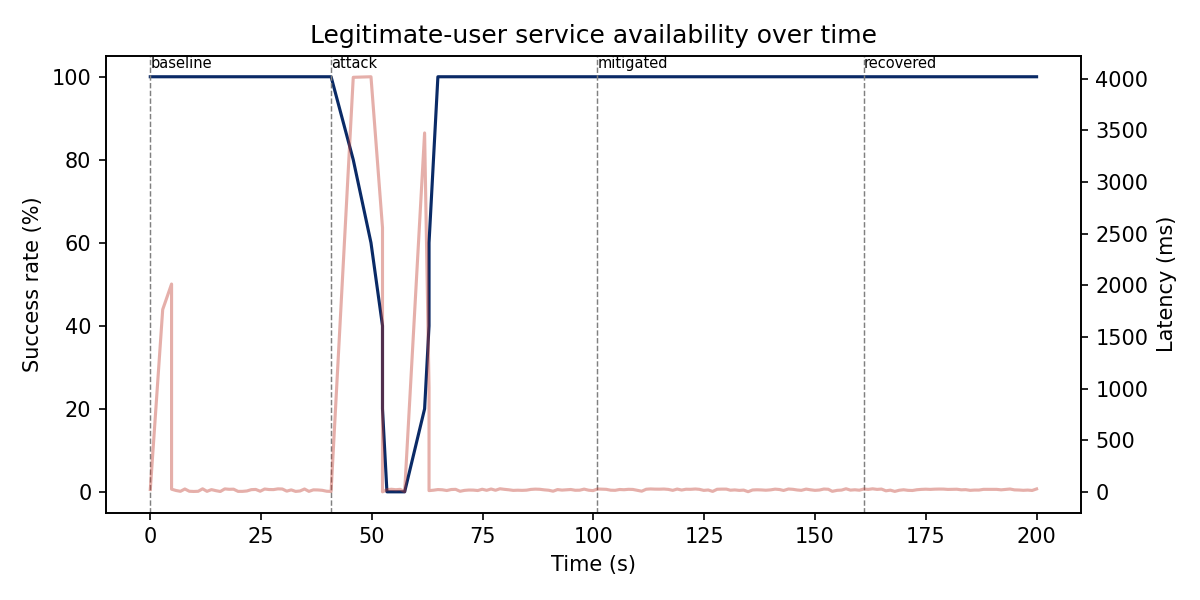
\includegraphics[width=\linewidth]{fig_availability.png}
\caption{Legitimate-user success rate and latency across the baseline, attack,
mitigated and recovered phases of the closed-loop experiment.}
\label{fig:avail}
\end{figure}

Table~\ref{tab:timing} decomposes the loop's responsiveness. Detection happens
within a single monitoring cycle of pool saturation; the mitigation ladder (reset,
drop, isolate) executes in roughly a second; the pool reclaim and the return of
legitimate traffic complete within a handful of seconds; and the automatic restore
fires one cooldown interval after the attack falls silent. The practical
consequence is that the service is unavailable only for the brief interval between
saturation and reclaim, rather than for the full duration of the attack as in the
undefended case.

\begin{table}[t]
\caption{Closed-loop timing and availability (measured).}
\label{tab:timing}
\centering
\footnotesize
\begin{tabular}{@{}lc@{}}
\toprule
Quantity & Value \\
\midrule
Baseline availability           & \RESavailBase\% \\
Availability during attack window & \RESavailAttack\% \\
Availability after mitigation    & \RESavailRecovered\% \\
Time-to-detect                   & $\le 1$ cycle ($\le\Delta$) \\
Time-to-mitigate (detect$\to$isolate) & $\approx 1$\,s \\
Time-to-recover (isolate$\to$service up) & a few seconds \\
Time-to-restore                  & one cooldown \\
False isolations of benign sources & 0 \\
Mitigation actions               & \RESnMitigations \\
\bottomrule
\end{tabular}
\end{table}

\subsection{RQ3: Overhead and comparison}
Fig.~\ref{fig:metrics} compares the models; the full adaptive loop adds the
isolate/restore behaviour on top of the best detector. The detector's monitoring
is lightweight---per-connection state and a single tree-ensemble inference every
two seconds---and runs comfortably alongside the service. The static-defense arm
(\texttt{mod\_reqtimeout}, a standard recommended control~\cite{owasp_dos}) is
evaded by an attacker trickling within the timeout window, so it does not by itself
prevent exhaustion; the closed loop, by
isolating the source, removes the pressure and lets the pool recover.

Concretely, the detector's recurring cost is one packet-capture callback per
observed segment plus, every $\Delta{=}2$\,s, one pass over the live flow table to
build feature vectors and a single batched tree-ensemble inference. Inference on a
few hundred flows with a depth-limited gradient-boosted model is sub-millisecond,
and the flow table is bounded by expiring idle flows, so memory stays flat under a
sustained attack. The monitor adds no latency to the data path---it observes a copy
of the traffic rather than proxying it---so the service's own request handling is
untouched except during the brief, deliberate reclaim. Against the undefended
baseline, where availability collapses to near zero for the full attack and stays
there, and against the static arm, which the attacker evades, the closed loop is the
only configuration that both detects the attack and returns the service to full
availability without operator action. The threshold-only arm detects saturation but,
lacking the completion feature, cannot attribute it to a specific source without
also implicating slow honest clients, which is precisely the false-isolation
failure our adaptive gate is designed to avoid.

\begin{figure}[t]
\centering
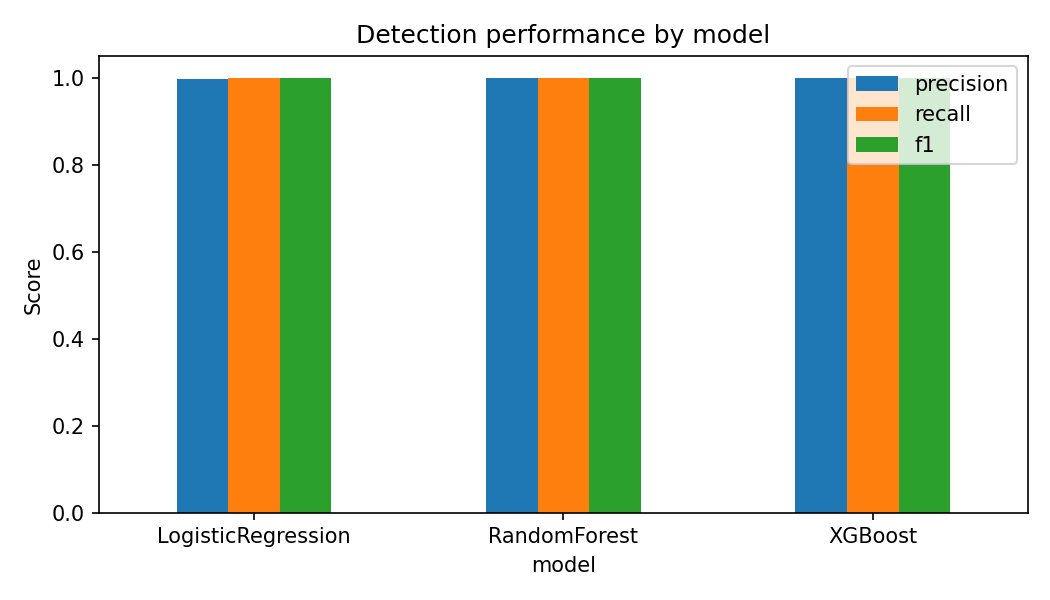
\includegraphics[width=\linewidth]{fig_metrics.png}
\caption{Precision, recall and F1 by model.}
\label{fig:metrics}
\end{figure}

\section{Discussion and Limitations}
The header-completion feature depends on reading request bytes, so it applies to
cleartext HTTP or to a TLS-terminating proxy; end-to-end-encrypted traffic blinds
this feature and would require TLS termination at the monitor. An adversary who
randomises timing (our jitter variant) stresses the inter-arrival features but
not header completion, which remains discriminative. The testbed is single-host;
distributed sources and cluster-wide isolation under
Kubernetes NetworkPolicy~\cite{k8s_netpol} are future work. Automated mitigation
carries a bounded risk of isolating a false positive; the saturation gate, the
duration gate, and the post-reclaim grace period together drove that risk to zero
in our runs, but the thresholds are deployment-specific and must be tuned.
Finally, the container-restart reclaim is a consequence of the test kernel
lacking \texttt{SOCK\_DESTROY}; on a production Linux host the mitigator would
force-close the attacker's sockets directly, avoiding even the brief restart.

\subsection{Relation to network-layer defenses}
SDN-based slow-DDoS mitigation~\cite{lukaseder2018sdn} shares our goal of acting on
slow attacks in real time, but operates at the network fabric and identifies
attackers from packet-rate and inter-arrival regularity alone. Our approach differs
in two ways that matter for containerized services. First, it reads the layer-7
completion state, which the fabric cannot see, and which is the most discriminative
signal against slow-but-honest clients. Second, its actuator is the container
runtime rather than switch flow rules, so the response is expressed in the same
vocabulary the platform already uses to manage tenants---disconnect this container,
restart that one---and composes naturally with existing orchestration. The two are
complementary: a fabric-level control could throttle a distributed source set while
the container-native loop protects the individual service and reclaims its pool.

\subsection{Operational considerations}
Three design choices make the loop safe to deploy. First, the saturation gate
ensures the system is inert while the service is healthy: no action is possible
unless the pool is genuinely under pressure, so a burst of slow honest clients on a
lightly-loaded server is never mitigated. Second, every action is reversible and
logged, and the cooldown guarantees that an isolation is lifted automatically once
the offending behaviour stops---there is no permanent block that an operator must
remember to clear. Third, the actions escalate from least to most disruptive, so
the cheapest effective remedy is tried first. The chief tuning burden is the
trio $(s_{\text{trig}}, k, d)$ of Table~\ref{tab:params}: too low and benign
bursts risk being flagged, too high and detection lags. In our environment the
values shown gave zero false isolations while keeping time-to-mitigate near one
second, but they should be re-fitted to a target service's pool size and traffic
profile.

\section{Conclusion and Future Work}
We presented a closed-loop, container-native defense against Slowloris that
monitors connection state, classifies flows with an adaptive-threshold XGBoost
detector, isolates offenders through the container runtime, reclaims the worker
pool, and restores service automatically---with a live dashboard that makes the
whole loop observable. The contribution is the automated loop, evaluated for
availability and responsiveness and shown to protect slow-but-honest clients, not
detection accuracy in isolation.

Several directions follow naturally. A Kubernetes deployment would replace
single-host container disconnection with NetworkPolicy-based isolation and
pod-level eviction, extending the loop from one host to a cluster and letting the
controller quarantine a compromised pod from its neighbours~\cite{k8s_netpol}.
Moving the monitor from user-space packet capture to eBPF would lower overhead and
allow line-rate feature extraction, making the approach viable for busier services.
Broadening the evaluation to the public CIC-IDS2017 and
CIC-DDoS2019~\cite{sharafaldin2018cicids,sharafaldin2019ddos} benchmarks would test
cross-dataset generalisation, and incorporating flash-crowd traces would attack the
harder discrimination problem the surveys highlight~\cite{deressu2026survey}.
Finally, the same loop should extend to the rest of the slow-DoS family---Slow POST,
Slow Read, and the HTTP/2 multiplexed variants~\cite{praseed2020http2}---since the
monitored invariants (duration, throughput, regularity, completion) are shared
across them, and to a TLS-terminating deployment so that the layer-7 features remain
observable on encrypted traffic.

\subsection{Threats to validity}
Our evaluation is on a single host with a single attacker, so the absolute timing
numbers reflect that scale; a distributed attack from many sources would stress the
per-source aggregation differently, though the per-flow features are unchanged. The
dataset is generated in our own environment, which controls labelling precisely but
is narrower than a public benchmark; we mitigate this by including genuinely slow
honest clients as hard negatives and by designing the methodology to admit
CIC-IDS2017 and CIC-DDoS2019. The near-perfect detection scores reflect a cleanly
separable two-class problem once the layer-7 feature is present and should not be
read as a claim that all application-layer DDoS is this easy; the harder, open
problem of flash-crowd discrimination~\cite{deressu2026survey} remains. Finally, the
specific reclaim mechanism is platform-dependent, as discussed.

\section{Reproducibility}
The entire testbed is defined declaratively in a single Docker Compose file and is
brought up with one command; a driver script collects the dataset, trains and
compares the models, runs the closed-loop defense experiment, and emits every
figure and table in this paper. The paper's numeric results are injected into the
manuscript automatically from the run outputs, so the reported figures cannot drift
from the experiment that produced them. The attack generator, detector, mitigator,
dashboard and analysis code, together with the exact configuration of
Table~\ref{tab:params}, constitute a complete package that a reader can re-run on a
single host with Docker installed.

\section*{Ethics Statement}
\label{sec:ethics}
All attacks were executed solely within an isolated laboratory network against a
self-hosted victim. The attack generator is restricted by an allow-list to the
laboratory subnet and refuses any other target. No external or third-party
systems were targeted at any point.

\bibliographystyle{IEEEtran}
\bibliography{references}

\end{document}
